\documentclass[12pt]{article}
\usepackage{setspace, graphicx, fullpage, amssymb, amsmath, epsfig, natbib, array, multirow, hyperref}
\usepackage{amsfonts, bm} 
\usepackage{dcolumn}
\usepackage{subfigure, float} 
\usepackage[margin=1in]{geometry} 
\usepackage{verbatim}
\usepackage{url}
\usepackage{enumerate}
\usepackage{morefloats}
\usepackage{caption}
\newcolumntype{d}[1]{D{.}{.}{#1}} 

\newcommand\fnote[1]{\captionsetup{font=small}\caption*{#1}}

\begin{document}

\section{Overview}

At our previous meeting we decided to:

\begin{itemize}
	
	\item Conduct further tests of differences between Senate classes in responsiveness
	
	\item Change the regression analysis in the paper to only have the all members of each chamber, with Senate models closer to those we use in the House
	
\end{itemize}

In the process of making changes to the regression models, I found that the current Senate data building script was failing to prevent retiring Senators from being marked as up for reelection. While models have been updated, this produced little substantive change in them. Models in the paper have been updated. Further, the differences design in this update (a visual of the test from last week's update) is shown with and without retirees included.

In any case, none of these look like things we want to show. While the change in responsiveness to party calls is greater in absolute terms for members in the 3rd Congress of their term, there are similarly sized differences between members in their 2nd Congress against those in their 1st. This does not invalidate our findings, by any means, but also does not do much to show more about the relationships we presently model in the paper.

Differences between coefficients with robust standard errors were insignificant at the 95\% one-tail threshold for both/. In the non-parametric tests (without retirees included), 87.9\% of the party call difference confidence interval of Congress 3-2 pairs fell below the estimate of the 2-1 pairs, and 81.3\% of the party call difference confidence interval of 3-1 pairs fell below the same estimate. In party free differences, 54.6\% of the 3-2 pairs' confidence interval fell below the 2-1 pair differences and 5.2\% of the 3-1 pair confidence interval fell below this threshold. I did not perform significance tests with the retiree pairs included.

\pagebreak

\section{Class Difference Coefficient Plots}

\begin{figure}[H]
	\centering
	\caption{Differences within Pairs, Retirees Included}
	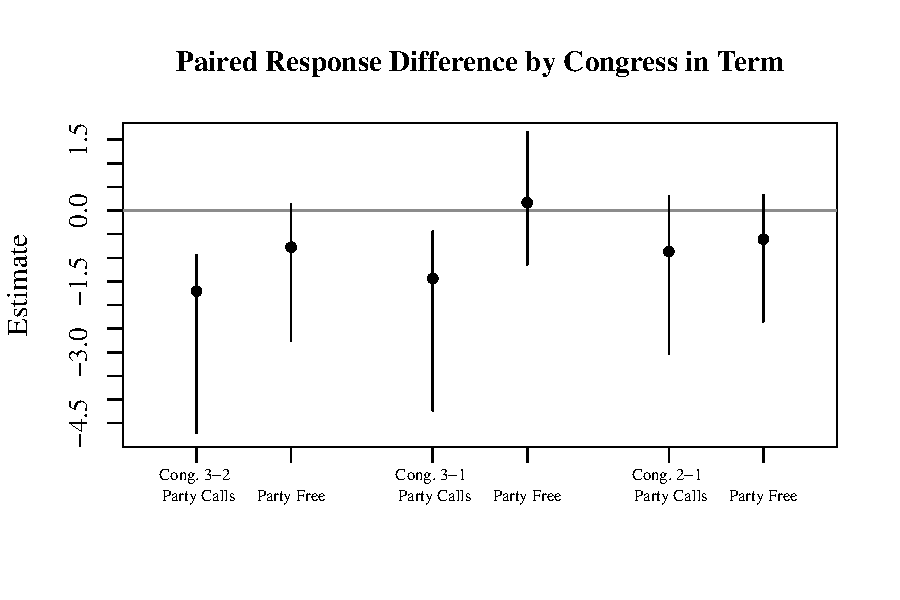
\includegraphics[width = 12cm]{C:/Users/Ethan/Documents/GitHub/partycalls/plots/diff_in_class_pair_retirees_included.pdf}
	\fnote{\textit{Note}: Results shown are produced by a paired-differences design among same state Senate pairs based on the Congress in their term. Higher Congresses are later in the term. Confidence intervals are produced by bootstrapping by Congress and state and represent the 95\% confidence range in a one-tailed test.}
\end{figure} 

\begin{figure}[H]
	\centering
	\caption{Differences within Pairs, Retirees Dropped}
	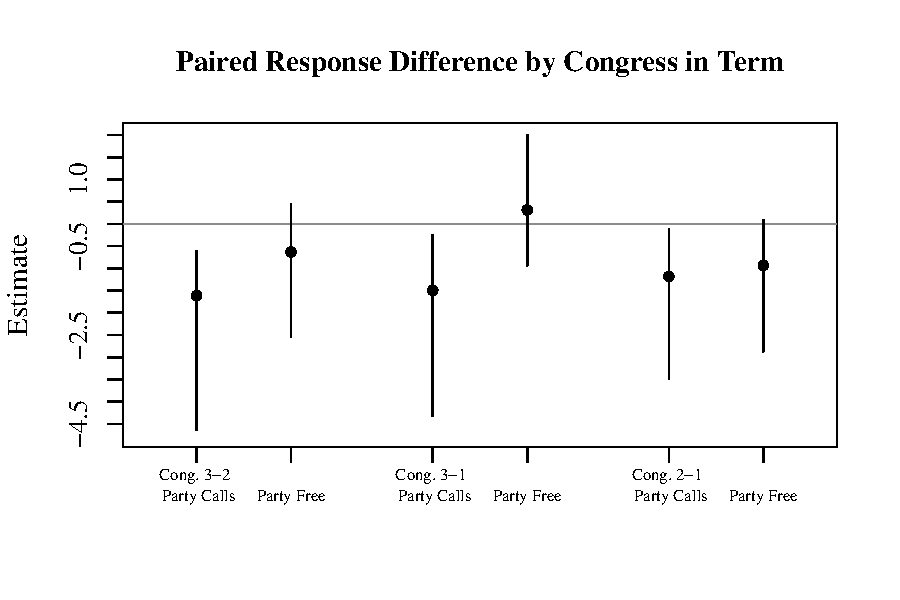
\includegraphics[width = 12cm]{C:/Users/Ethan/Documents/GitHub/partycalls/plots/senate_diff_pairs.pdf}
	\fnote{\textit{Note}: Results shown are produced by a paired-differences design among same state Senate pairs based on the Congress in their term. Higher Congresses are later in the term. Confidence intervals are produced by bootstrapping by Congress and state and represent the 95\% confidence range in a one-tailed test.}
\end{figure} 

\begin{figure}[H]
	\centering
	\caption{Regression Coefficients with Robust Standard Errors: Class Pair Type}
	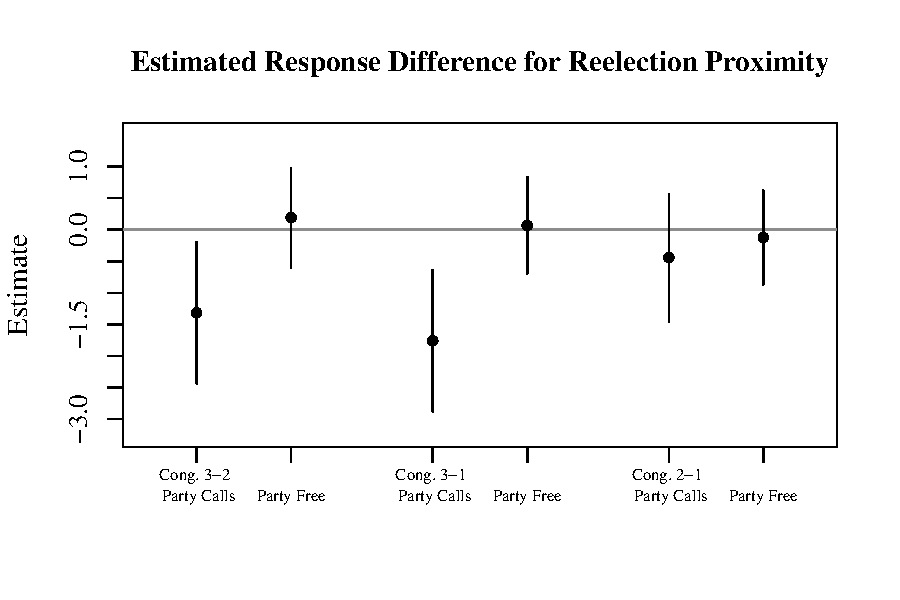
\includegraphics[width = 12cm]{C:/Users/Ethan/Documents/GitHub/partycalls/plots/senate_reelection_robust_se.pdf}
	\fnote{\textit{Note}: Results shown are produced by regressions with rate of voting with the majority of one's party on party call votes and party free votes in the Senate. Results were separately estimated for members of Congress based on their place in their term in order to compare aggregate response rate differences between those closer to and further from reelection. Senators who retired during or at the end of a Congress are excluded from the analysis. Estimates are shown with robust standard errors providing 95\% one-tail confidence intervals.}
\end{figure}

\begin{figure}[H]
	\centering
	\caption{Regression Coefficients with Robust Standard Errors: Class Pair Interaction, Party Calls}
	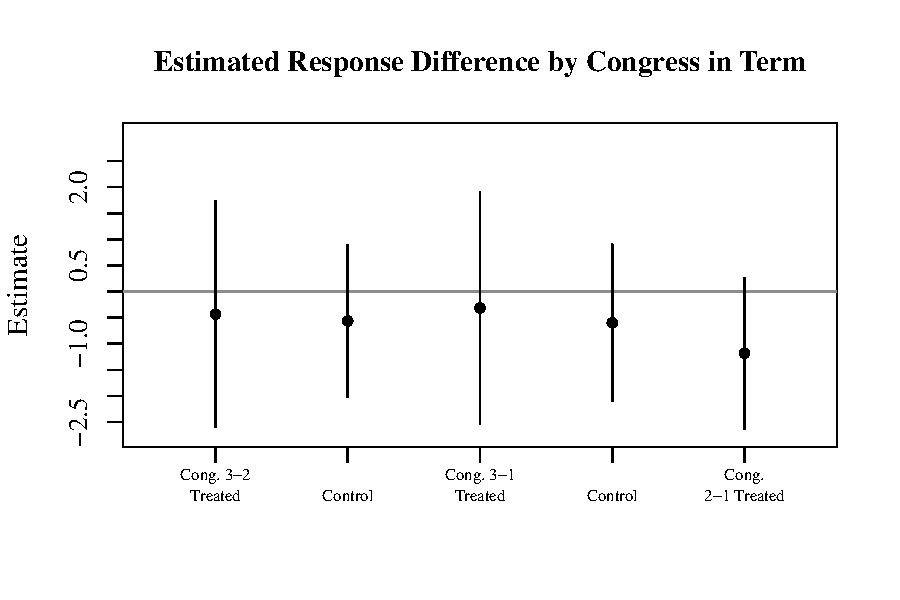
\includegraphics[width = 12cm]{C:/Users/Ethan/Documents/GitHub/partycalls/plots/senate_reelection_interaction_pi_robust_se.pdf}
	\fnote{\textit{Note}: Results shown are produced by regressions with rate of voting with the majority of one's party on party call votes in the Senate. Results shown were estimated by interacting an indicator for the relative place in terms of the pair of same-state Senators. Estimates are shown with robust standard errors providing 95\% one-tail confidence intervals.}
\end{figure}

\begin{figure}[H]
	\centering
	\caption{Regression Coefficients with Robust Standard Errors: Class Pair Interaction, Party Free}
	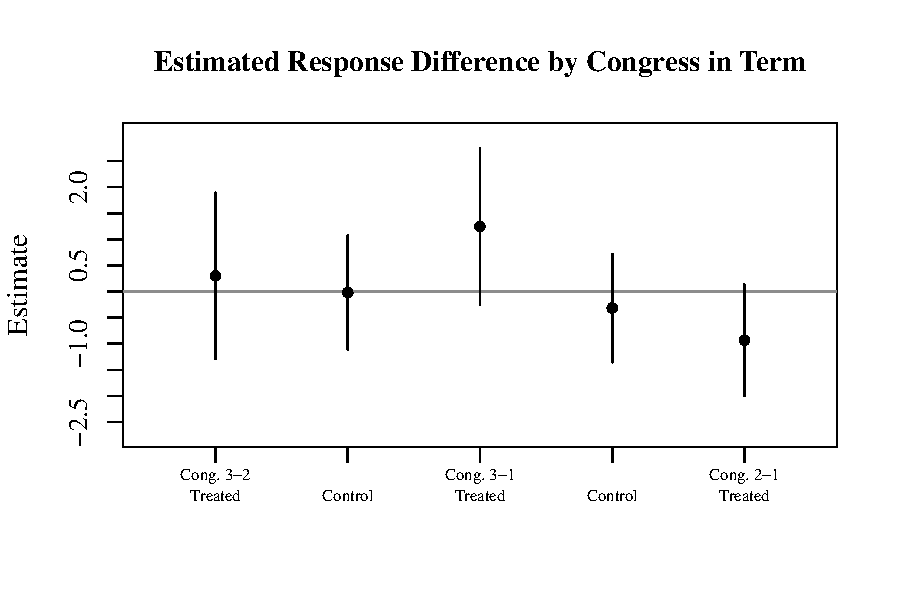
\includegraphics[width = 12cm]{C:/Users/Ethan/Documents/GitHub/partycalls/plots/senate_reelection_interaction_pf_robust_se.pdf}
	\fnote{\textit{Note}: Results shown are produced by regressions with rate of voting with the majority of one's party on party free votes in the Senate. Results shown were estimated by interacting an indicator for the relative place in terms of the pair of same-state Senators. Estimates are shown with robust standard errors providing 95\% one-tail confidence intervals.}
\end{figure}




\end{document}